\documentclass[a4paper,12pt]{article}

\usepackage[T1]{fontenc}
\usepackage{times}
\usepackage[swedish,english]{babel}
\usepackage[utf8]{inputenc}
\usepackage{dtklogos}
\usepackage{wallpaper}
\usepackage[absolute]{textpos}
\usepackage[top=2cm, bottom=2.5cm, left=3cm, right=3cm]{geometry}
\usepackage{appendix}
\usepackage[nottoc]{tocbibind}
%\usepackage{setspace}

\setcounter{secnumdepth}{3}
\setcounter{tocdepth}{3}

\usepackage{sectsty}
\sectionfont{\fontsize{14}{15}\selectfont}
\subsectionfont{\fontsize{12}{15}\selectfont}
\subsubsectionfont{\fontsize{12}{15}\selectfont}

\usepackage{csquotes} % Used to handle citations
\renewcommand{\thetable}{\arabic{section}.\arabic{table}}  
\renewcommand{\thefigure}{\arabic{section}.\arabic{figure}}

%----------------------------------------------------------------------------------------
%	
%----------------------------------------------------------------------------------------
\newsavebox{\mybox}
\newlength{\mydepth}
\newlength{\myheight}

\newenvironment{sidebar}%
{\begin{lrbox}{\mybox}\begin{minipage}{\textwidth}}%
{\end{minipage}\end{lrbox}%
 \settodepth{\mydepth}{\usebox{\mybox}}%
 \settoheight{\myheight}{\usebox{\mybox}}%
 \addtolength{\myheight}{\mydepth}%
 \noindent\makebox[0pt]{\hspace{-20pt}\rule[-\mydepth]{1pt}{\myheight}}%
 \usebox{\mybox}}

%----------------------------------------------------------------------------------------
%	Title section
%----------------------------------------------------------------------------------------
\newcommand\BackgroundPic{
    \put(-2,-3){
    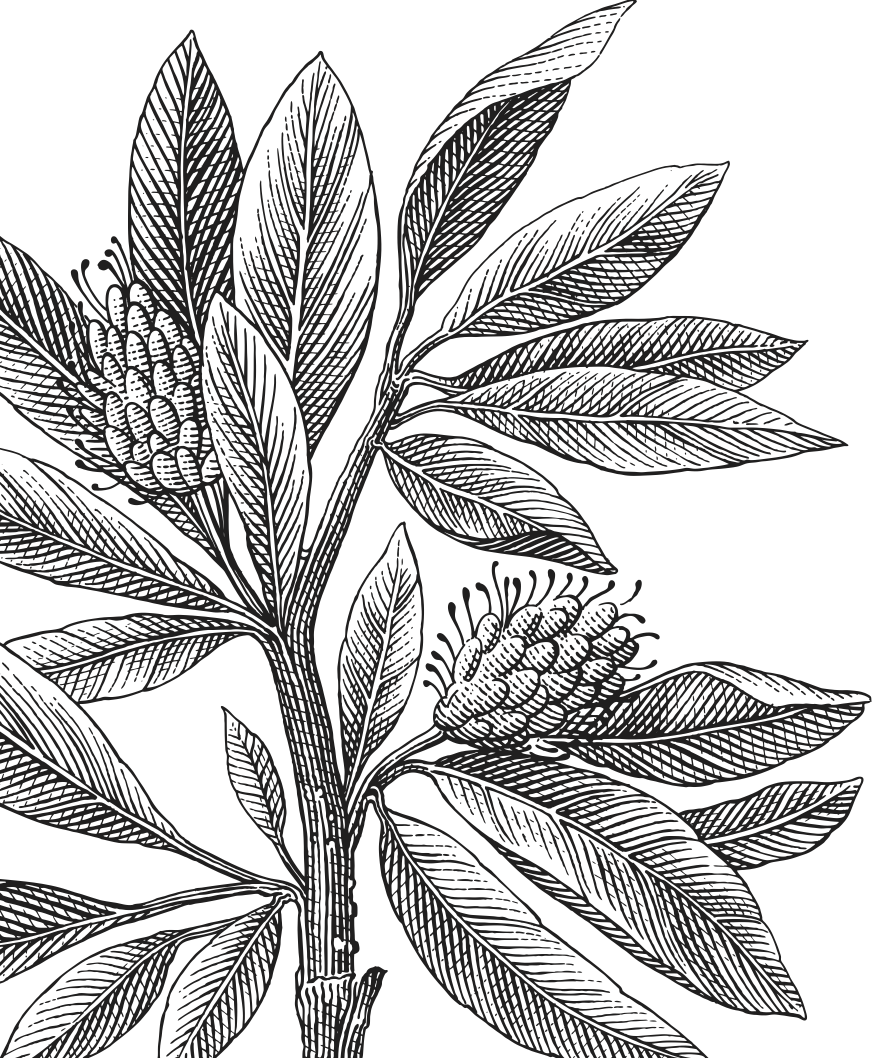
\includegraphics[keepaspectratio,scale=0.3]{img/lnu_etch.png} % Background picture
    }
}
\newcommand\BackgroundPicLogo{
    \put(30,740){
    
\includegraphics[keepaspectratio,scale=0.10]{img/logo.png} % Logo in upper left corner
    }
}

\title{	
\vspace{-8cm}
\begin{sidebar}
    \vspace{10cm}
    \normalfont \normalsize
    \Huge Assignment 1: Jodel Alert \\
    \vspace{-1.3cm}
\end{sidebar}
\vspace{3cm}
\begin{flushleft}
    \huge Software Engineering - Design\\ 
    \it \LARGE - 2DV603
\end{flushleft}
\null
\vfill
\begin{textblock}{6}(10,12)
\begin{flushright}
\begin{minipage}{\textwidth}
\begin{flushleft} \large
\emph{Name:} Patrik Hermansson\\ % Author
\emph{Email:} ph222md@student.lnu.se\\
\emph{Name:} Michael Wagnberg\\ % Author
\emph{Email:} mw222uu@student.lnu.se\\
\emph{Name:} Benjamin Svärd\\ % Author
\emph{Email:} bs222et@student.lnu.se\\
\emph{Name:} Christofer Nguyen\\ % Author
\emph{Email:} cn222hn@student.lnu.se\\
\emph{Name:} Jonathan Walkden\\ % Author
\emph{Email:} jw222qi@student.lnu.se\\
\end{flushleft}
\end{minipage}
\end{flushright}
\end{textblock}
}

\date{} 
\newpage
\begin{document}
\pagenumbering{gobble}
\newgeometry{left=5cm}
\AddToShipoutPicture*{\BackgroundPic}
\AddToShipoutPicture*{\BackgroundPicLogo}
\maketitle
\restoregeometry
\selectlanguage{english}
\pagenumbering{gobble}
\newpage
\tableofcontents % Table of contents
\pagenumbering{arabic}
\newpage
\section{Domain Analysis Document}
\subsection{Introduction, Problem and Background}
Words from our customer:\\

Jodel is a new anonymous social app targeting students
and campus life. Some questions and comments posted
there are specifically related to things that the Student
Union deal with, i.e. questions about accommodation,
what rules apply when writing an exam, if you need a
student ID to get into the pubs etc. 

We’d love to
comment on such questions, but they are far between
and we haven’t got time to monitor the feeds so if
possible it would be great to have functionality that
could tap into the Jodel API and send e-mail alerts if
relevant keywords show up; similar to Google Alerts or
Meltwater.
\\

We are supposed to create an application that will listen for keywords entered in posts in the Jodel application, and when keyword found an email will be generated and sent to Linnéstudenterna. They will then know that a post has been made that regards Linnéstudenterna and can act upon. The basic idea is to just get this functionality to work.\\
A desiderata for our customer is that they should also be able to add/delete and edit keywords as well as recipient email, so that they can tailor the application after their needs.
\subsection{General knowledge about the domain}
The generald field of business for Linnéstudenterna is to represent students att Linneaus University and to make the time at the university as good as possible. They help with advices, support or if someone have been treated wrongly or unjustly by the university, as well as discounts and contact with commercial and industry life. They are not a technology company but they want to use technology in order to connect more with the students.
\subsection{Customers and users}
The customers of Linnéstudenterna are the users of Jodel. Our customer/stakeholder is Linnéstudenterna. Our customer has ordered an application to handle relationship with the students asking questions on Jodel.
\subsection{Environment}
The environment used will be a PC running Windows which the application will be run upon on. This computer must be up and running and online twenty-four seven in order for the application to work properly. A mail-server will run in the background of the application which will send email to the chosen recipients in case of a registered keyword gets posted.\\
Application will be written and developed in Java. This makes it versatile and can work on all platforms needed.
\\The application Jodel is already in place and we are going to base our work around the API of that program and create a new application. Nothing else is in place, there is no half-done project that covers this problem, so everything will be created from scratch.
If the API is not accessible, we are going to use mitmproxy to listen to the traffic and save data which we can process in order to produce the required email.
\subsection{Tasks and procedures currently performed}
Today Linnéstudenterna manually checks Jodel from time to time in order to capture some of the questions and answering them, but this is too time consuming and there is no way they can monitor the feed all the time. They currently do not use any technology in aid other than the app itself.
\subsection{Competing software}
Jodel is kind of alone on the market with its nische, and tapping on to their feed in order to capture keywords is not something that exists right now.
Other software that taps into feeds and derives statistics and data are Google Alert and Meltwater.
\subsection{Product placement}
This application can be used by Linnéstudenterna in order to connect with the students when they have questions. Other aspects that this application can cover can also be in the commercial market. \\
Companies can tap in and scan the feed and see what is said about that company, and because Jodel is an anonymous application, people tend to say the truth, or completely the opposite. This can build a knowledge about the customers using a specific brand or a chain and companies can act upon that information in marketing campaigns or changing the way they act against customers.
\subsection{Stakeholder's vision for the future}
Our stakeholder's desiderata is to have a web based interface with functions like managing keywords and emails, and this application can be a start of something bigger in the future with more added functionality.
Our customer want to be able to answer to a post directly from the web interface.

\section{Problem}

\section{Background information}

\section{Environment and system models}

\begin{figure}[!h]
	\centering
	
\includegraphics[height=6cm]{img/jodel.png}
	\caption{Jodel logo}
	\label{Cisco routing}
\end{figure}
\section{Functional requirements}
\begin{enumerate}
	\item When a keyword is used in a Jodel post, Linnestudenterna will receive a mail
	\item The application will request Jodel posts.
	\item Keywords should be able to be removed
	\item Keywords should be able to be added
	\item Keywords should be able to be changed
	\item Added keywords saved between sessions (i.e saved on local host if you restart the app)
	\item Recipient email should be able to be removed
	\item Recipient email should be able to be added
	\item Recipient email should be able to be changed
\end{enumerate}
\section{Non-functional requirements}
\begin{enumerate}
	\item App will continuously scan Jodel traffic every 15 minutes.
	\item When a keyword has been found, email should be sent within 2 seconds
\end{enumerate}
\section{Participating Objects}
Domain model containing the participating objects.\\

\begin{figure}[!h]
	\centering
	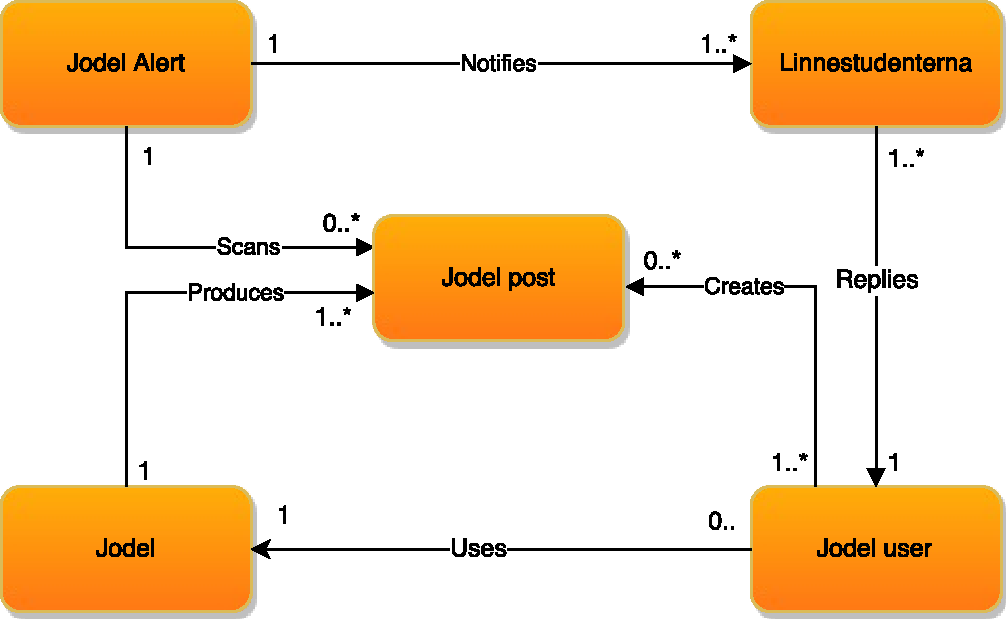
\includegraphics[height=9cm]{img/ParticipatingObjects.pdf}
	\caption{Jodel logo}
	\label{Cisco routing}
\end{figure}

\end{document}